\documentclass{beamer}
\usepackage{etex}

\usetheme{KTHprofile}

\title{Mutli agent control with LTL specifications and abstraction with input memories}
\subtitle{Master thesis 2016}
\author{Paul Rousse}
\institute{Automatic Departement}
\date{\today}


\usepackage{graphicx}
\graphicspath{{./plots/}{./env/}{./results/}{./pres/}}
\usepackage[mode=buildnew]{standalone}
\usepackage{epstopdf}
\usepackage[absolute,overlay]{textpos}
\usepackage{tikz}
\usetikzlibrary{shapes,arrows,calc}
\usepackage{pgfplotstable} % For \pgfplotstableread


%% MATH
\usepackage{amsmath, amsfonts, amsthm, amssymb}
\usepackage{nicefrac}
\usepackage{breqn}
\usepackage{tabularx}
\usepackage{stmaryrd} % for llbracket and rrbracket
\usepackage[ruled]{algorithm2e}

% LTL temporal operator
\DeclareFontFamily{U}{matha}{\hyphenchar\font45}
\DeclareFontShape{U}{matha}{m}{n}{
      <5> <6> <7> <8> <9> <10> gen * matha
      <10.95> matha10 <12> <14.4> <17.28> <20.74> <24.88> matha12
      }{}
\DeclareSymbolFont{matha}{U}{matha}{m}{n}
\DeclareMathSymbol{\vDash}{3}{matha}{'52}
\DeclareMathSymbol{\nvDash}{3}{matha}{'50}

\DeclareMathOperator*{\argmin}{arg\,min}
\makeatletter
\newcommand{\tuple}[1]{
	\@tempcnta=0
	\def\mylist{#1}
	\@for\next:=\mylist\do{
	\ifnum \@tempcnta = 0 \else ,\linebreak[1]\fi \next
	\advance\@tempcnta\@ne}
}
\makeatother

%\renewcommand{\splitatcommas}[1]{#1}

\newcommand{\buchi}[0]{B\"uchi}

%% LTL symbols defintion
\usepackage{latexsym} % get the right \Diamond symbol
\newcommand{\LTLalways}		{\ensuremath{\square}}
\newcommand{\LTLeventually}	{\ensuremath{\Diamond}}
\newcommand{\LTLuntil}		{\ensuremath{\mathsf{U}}}
\newcommand{\LTLnext}		{\ensuremath{\bigcirc}}
\newcommand{\LTLimply}			{\ensuremath{\rightarrow}}
\newcommand{\true}			{\ensuremath{\top}}
\renewcommand{\and}			{\ensuremath{\wedge}}


\newcommand{\outpost}{ \ensuremath{\overline{Post} } }
\newcommand{\inpre}{ \ensuremath{\overline{Pre} } }

%% MATH COMMANDS
\newcommand{\vect}[1]{\ensuremath{ \mathbf{#1}}}
\newcommand{\leftint}{\left \llbracket}
\newcommand{\rightint}{\right \rrbracket}
\newcommand{\abs}[1]{\left|#1\right|}
\newcommand{\card}[1]{\left|#1\right|}


\usepackage{tikz}
\usetikzlibrary{shapes.geometric, arrows, positioning, calc, fit, arrows, decorations.pathreplacing,patterns}
\usepackage{pgfplots}
\usepgfplotslibrary{groupplots,fillbetween}
\usepackage{relsize}


%% TRANSITION SYSTEM COMMANDS
\usepackage[all]{xy}
\usepackage{amssymb}
\newdir{|>}{-{\scriptscriptstyle{\blacktriangleright}}}
\newcommand{\transition}{
  \ensuremath{ \xymatrix{\ar@{-|>}[r]&} }
  }
\newcommand{\labelledtransition}[1]{
  \ensuremath{ \xymatrix{\ar@{-|>}[r]^{#1}&} }
  }
\newcommand{\systransition}[2]{
  \ensuremath{ \xymatrix{\ar@{-|>}[r]^{#2}_{#1}&} }
  }

\newcommand{\Post}[2]{Post_{#2}^{#1}}
\newcommand{\Reach}[2]{Reach^{#1}({#2})}
\newcommand{\ReachSeq}[2]{Reach^{*#1}(#2)}

\newcommand{\sysDef}[1]{(\)}

\newcommand{\altsim}{\preceq_{\mathcal{AS}}}
  

\newcommand{\T}[1]{#1{}^\top}
\newcommand{\proj}[1]{|_{#1}}

\renewcommand{\exp}[1]{e^{#1}}



\newcommand{\SSunobs}{\mathfrak{X}^i}
\newcommand{\SSobs}{\mathfrak{X}^o}
\newcommand{\Ninputs}{\Delta n_u}%
\newcommand{\y}{\vect{y}}%
\newcommand{\x}{\vect{x}}%
\newcommand{\xa}{\vect{x}^a}%
\newcommand{\xobs}{\vect{x}^o}%
\newcommand{\Xobs}{X^o}%
\newcommand{\Xobsinit}{X^o_0}%
\newcommand{\xunobs}{\vect{x}^i}%
\newcommand{\Xunobs}{X^i}%
\newcommand{\Sunobs}{\mathcal{S}^i}%
\newcommand{\Xuinv}{{\mathcal{X}^i}}%
\newcommand{\pastuseq}{\vect{u}_{n-\Ninputs},\dots,\vect{u}_{n-1}}%
\newcommand{\pastuseqn}{\vect{u}_{n+1-\Ninputs},\dots,\vect{u}_{n}}%
\newcommand{\Pastuseq}{U_n}%
\newcommand{\sys}{\mathcal{S}}%
\newcommand{\sysa}{\mathcal{S}_a}%
\newcommand{\sysaU}{\mathcal{U}}%
\newcommand{\sysA}{\mathcal{S}_A}%
\newcommand{\sysB}{\mathcal{S}_B}%
\newcommand{\sysC}{\mathcal{S}_C}%
\newcommand{\Usys}{\mathcal{U}}%
\newcommand{\Wsys}{\mathcal{W}}%
\newcommand{\Uunobs}{{\mathcal{U}^i}}%
\newcommand{\Wunobs}{{\mathcal{W}^i}}%
\newcommand{\uobs}{\vect{u}^o}%
\newcommand{\wobs}{\vect{w}^o}%
\newcommand{\uunobs}{\vect{u}^i}%
\newcommand{\wunobs}{\vect{w}^i}%
\newcommand{\Dunobs}{n^i}% Dimension of the ss of unobs
\newcommand{\R}{\mathbb{R}}% real set
%%
% Monotone systems
\newcommand{\mle}{\prec}
\newcommand{\mleq}{\preceq}
\newcommand{\minf}[1]{\underline{#1}}
\newcommand{\msup}[1]{\overline{#1}}
%%
% linear system
\newcommand{\X}{X}%
\newcommand{\Xinv}{\mathcal{X}}%
\newcommand{\U}{\mathcal{U}}%
\newcommand{\W}{\mathcal{W}}%
\newcommand{\vu}{\vect{u}}%
\renewcommand{\u}{\vect{u}}%
\renewcommand{\U}{\mathcal{U}}%
\newcommand{\w}{\vect{w}}%
\newcommand{\s}{\vect{s}}%
\newcommand{\st}{\vect{t}}%
%
% Continuous model
\newcommand{\traj}{\varphi}
%
% discretization of the abstraction
\newcommand{\xd}{\x_d}
\newcommand{\vd}{\vect{v}_d}
\newcommand{\Nobs}{N^o} % number of states of the discretization of the state space \SSobs
%
\newcommand{\dt}{dT}%

\begin{document}

\begin{frame}
\titlepage
\end{frame}


%% INTRO
\section{Introduction}

% Introduct with the project, wind turbine
%	- what do we want to achieve: motion planning 
%	- what are the specifications: collision avoidance between the agents
%	- one solution: -> using formal methods in order to do this
\begin{frame}
\frametitle{Wind turbine maintenance scenario}

\begin{figure}
\begin{minipage}{0.2\textwidth}
\centering

\includegraphics[width=\textwidth]{aerowork}
\end{minipage}
\hspace*{\fill}%
\begin{minipage}{0.5\textwidth}
\centering
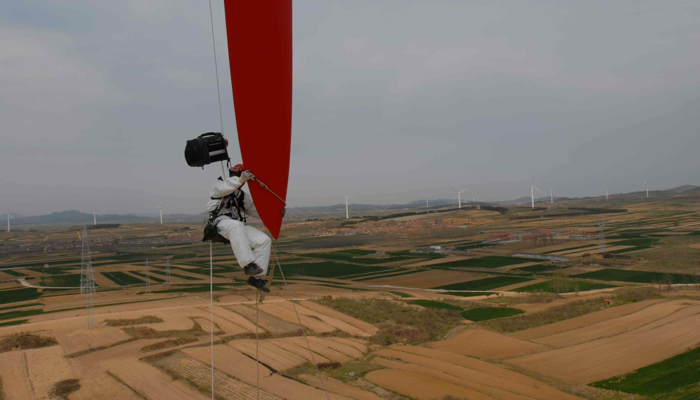
\includegraphics[width=\textwidth]{windturbine}
\end{minipage}
\end{figure}

\begin{itemize}
\item Motion and task specifications
\item Safety requirements (avoid collision, stay inside a safety area)
\end{itemize}

\end{frame}


\begin{frame}
\frametitle{Outline}
\tableofcontents
\end{frame}


\section{Preliminaries}
% Describe how does these methods works, the different steps in order to build the controller


\newcommand{\planframe}[1]{
\begin{frame}
\begin{figure}
\def\framenbre{#1}
\includestandalone[width=\textwidth]{diagram_pres}
\end{figure}
\end{frame}
}

\planframe{0}

\subsection{Temporal logic}
%info: first you talk about how you will give this specifications (to say that they will be given in a automaton form, this justify the fact that we try to find an abstractino of the system in the form of a finite transition system)

% LTL, conversion to a buchi automaton, explain what are the conditions so that a path is accepted in the buchi automaton and what it means on the LTL formula
\begin{frame}
\frametitle{High level specification: the temporal logic}
\begin{block}{Linear temporal logic (LTL)}
$$ \varphi ::= 
\true \mid 
a \mid 
\varphi_1 \land \varphi_2 \mid
\lnot \varphi \mid
\LTLnext \varphi \mid
\varphi_1 \LTLuntil \varphi_2$$
\end{block}
\pause

\begin{block}{\buchi{} Automaton}

\end{block}

\begin{figure}
\begin{minipage}{0.45\textwidth}
$\varphi = \LTLalways \LTLeventually a$
\end{minipage}
{\LARGE$\Rightarrow$}%
\begin{minipage}{0.45\textwidth}
\hspace*{1cm}
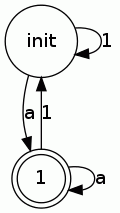
\includegraphics[width=1.5cm]{buchi}
\end{minipage}
\end{figure}

\end{frame}

\planframe{1}

\subsection{Abstraction}
% abstractions methods (unfiorm discretization)
\begin{frame}
\frametitle{Abstraction}

\begin{figure}
\centering
\begin{minipage}{.45\textwidth}
  \centering
  \includestandalone[width=\linewidth]{state_space_repr}
  \caption{Model of the robot}
\end{minipage}
{\LARGE$\rightarrow$}%
\begin{minipage}{.45\textwidth}
  \centering
\tikzstyle{nodestyle} = [draw,circle]
\tikzstyle{trans} = [->]
\tikzstyle{labelcont} = [pos=0.7,inner sep = 1pt]
\resizebox {0.7\columnwidth} {!} {
\begin{tikzpicture}[node distance = 1cm, auto]
    % Place nodes
    \node [nodestyle] (n1) {n1};
    \node [nodestyle,right of=n1,yshift=2.5cm,xshift=2cm] (n2) {n2};
    \node [nodestyle,below of=n2] (n3) {n3};
    \node [nodestyle,below of=n3] (n4) {n4};
    \node [nodestyle,below of=n4] (n5) {n5};
    \node [nodestyle,below of=n5] (n6) {n6};
    \node [nodestyle,below of=n6] (n7) {n7};
    
    \newcommand{\cont}{$\mathbf{u}_n$}
    
    \draw [trans] (n1) -- node[labelcont] {\cont} (n2);
    \draw [trans] (n1) -- node[labelcont] {\cont} (n3);
    \draw [trans] (n1) -- node[labelcont] {\cont} (n4);
    \draw [trans] (n1) -- node[labelcont] {\cont} (n5);
    \draw [trans] (n1) -- node[labelcont] {\cont} (n6);
    \draw [trans] (n1) -- node[labelcont] {\cont} (n7);
\end{tikzpicture}
}
\caption{Finite Transition System}
\end{minipage}
\end{figure}

\end{frame}


\planframe{2}

\subsection{Controller synthesis}

\begin{frame}
\frametitle{Controller synthesis}

\begin{block}{Solution plan}
Every path in the product automaton going infinitely often to the goal set verify the LTL formula and the dynamical system behavior.
\end{block}

$\Rightarrow$ Controller =  $\{(q_1,u_1),(q_2,u_2), \dots, (q_n,u_n)\}$

\end{frame}


\planframe{3}
\planframe{5}

%% PLAN
%% Present a rough plan of what you did:
%	- abstraction
%	- algorithm used

%% ABSTRACTION
\section{State extended abstraction}
% abstraction of the quadricopter, talk about the transient state that belong to the second integrator model, the complexity of the second integrator model
% bring the solution of the input memories
% explain the steps to build the abstraction
% show that the actual admissible noise is bigger set (give the formula to get the equation and the bode diagram of it)
\newcommand{\vv}{\mathbf{v}}
\begin{frame}
\frametitle{State extended abstraction}
Dynamical system: $(\x^o,\x^i) 
\systransition{S}{\u}
 (\x^o_+,\x^i_+)$
 
Abstraction: $(\x^o,\u_{n - \Ninputs},...,\u_{n-1}) 
\systransition{S_a}{\u}
 (\x^o_+,\u_{n+1-\Ninputs},...,\u_{n-1},\u)$
\pause
\begin{figure}
\includestandalone[width=\textwidth]{abstraction_process_2}
\end{figure}
\end{frame}

\begin{frame}
\frametitle{Comparison with uniform discretization}

\begin{figure}
\begin{minipage}{0.4\textwidth}
\includestandalone[width=\linewidth]{state_space_repr}
\end{minipage}
\begin{minipage}{0.4\textwidth}
\includestandalone[width=\textwidth]{feasible_models}
\end{minipage}
\end{figure}

\only<1>{
\begin{equation*}
\begin{split}
\dot{\vv} &= k (\vv_{ref} - \vv) + \w_v\\
\dot{\x} &= \vv + \w_x\\
\varphi &= (\LTLalways \LTLeventually a) \and (\LTLalways \LTLeventually b) 
\end{split}
\end{equation*}
}

\only<2->{
\begin{itemize}
\item more conservative (the information is selected more wisely)
\pause
\item less reachable
\end{itemize}
}
\end{frame}

\begin{frame}
\frametitle{Admissible noise}

\begin{figure}
\begin{minipage}{0.45\textwidth}
\centering
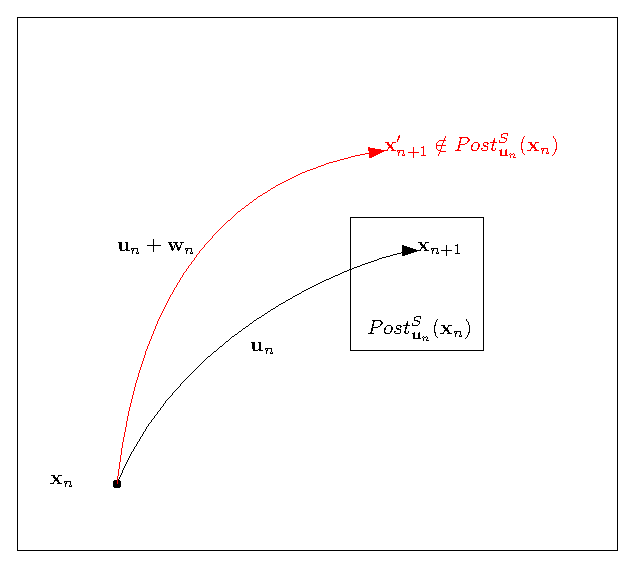
\includegraphics[width=\textwidth]{noise_1}
\caption{Dynamical system}
\end{minipage}
\pause
\begin{minipage}{0.45\textwidth}
\centering
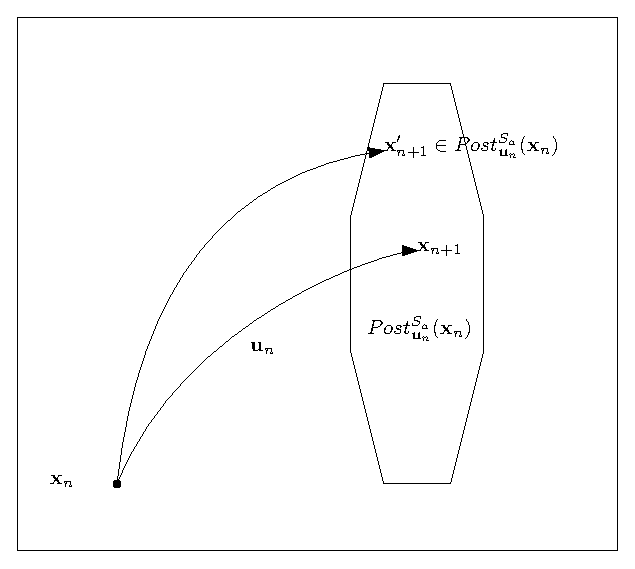
\includegraphics[width=\textwidth]{noise_2}
\caption{Abstraction}
\end{minipage}
\end{figure}

\end{frame}

\begin{frame}
\frametitle{Admissible noise}

$\mathcal{W}_a = \{ \{\w_n\}_{n\in\mathbb{N}}  \mid \mathcal{L}_1(G \ast G_{\w} ) \leq \sigma \}$

$\mathcal{W} \subset \mathcal{W}_a$

\begin{figure}
\begin{minipage}{0.45\textwidth}
\centering
\includestandalone[width=\textwidth]{bode_plots}
\end{minipage}
\begin{minipage}{0.45\textwidth}
\centering
\includestandalone[width=\textwidth]{speed_plots_reachables_sets}
\end{minipage}
\end{figure}

\end{frame}

%% ALGORITHM
% explain what was the trouble (take in account non determinism of the model)
\begin{frame}
\frametitle{Path planning algorithm}

Planning domain:
\begin{itemize}
\pause
\item Non deterministic FTS
\pause
\item Self-loops and cycles
\end{itemize}

Classic algorithms:
\begin{itemize}
\pause
\item
\pause
\item Self-loops and cycles
\end{itemize}

\end{frame}

% talk mabout the conditions of the buchi automaton and what is not nice with non determinism / self loops -> introduce the fairness property.

% present the plan decomposition,
\newcommand{\onlyframe}[2]{%
\only<#1>{%
\def\framenbre{#2}%
\includestandalone[width=0.5\textwidth]{plan_decomposition_beamer}%
}}
\begin{frame}
\frametitle{Plan decomposition - $\varphi = \LTLeventually G$}
\begin{figure}
\onlyframe{1}{2}%
\onlyframe{2}{3}%
\onlyframe{3}{4}%
\onlyframe{4}{5}%
\onlyframe{5}{6}%
\onlyframe{6}{7}%
\end{figure}

\end{frame}
% say that you have created a backward reachability alogirthm that go through the solution and check if the controller configuration is fair


%% EXPERIMENTS
% show the video of the multi agent experiment
\begin{frame}
\frametitle{Experiments}
\end{frame}



\begin{frame}
\frametitle{Multi agent experiment}
\begin{itemize}
\item 0 memories (equivalent to the first integrator model)
\item $\varphi = (\LTLalways \neg out) \and (\LTLalways \LTLeventually a) \and (\LTLalways \LTLeventually b) \and (\LTLalways \neg collide)$
\end{itemize}

\begin{figure}
  \begin{minipage}{0.3\textwidth}
    \centering
    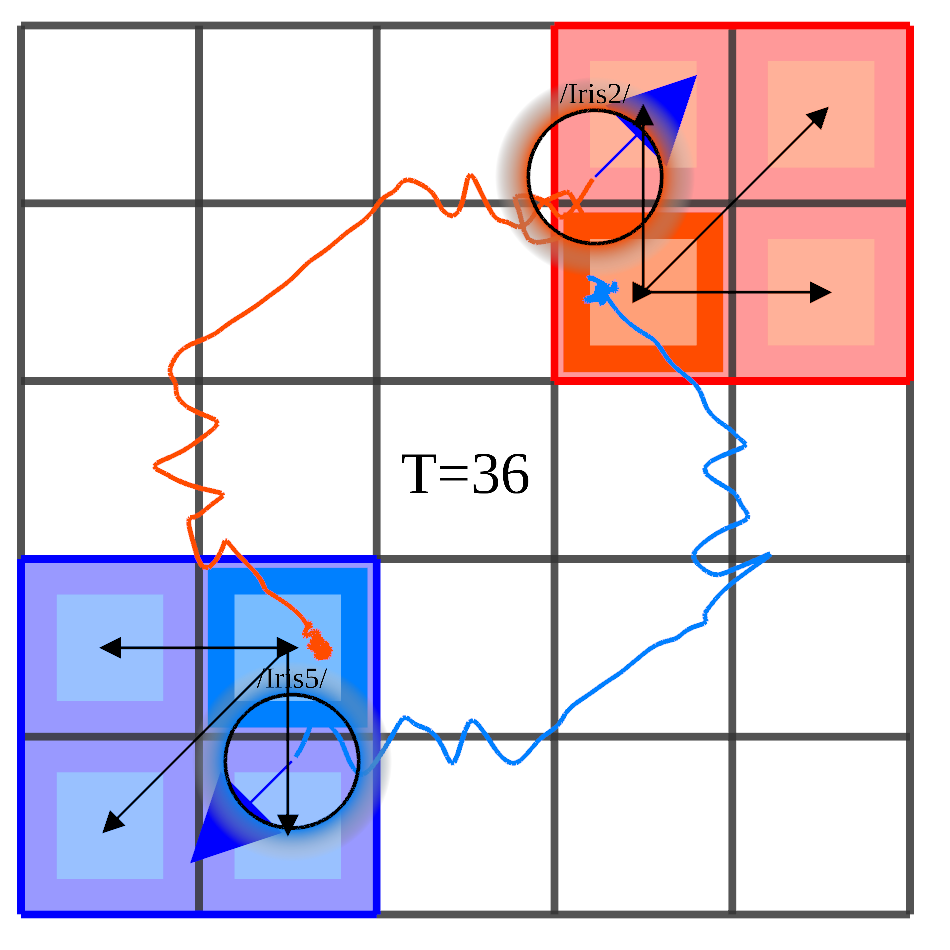
\includegraphics[width=\linewidth]{multi_ltl/multi11}
  \end{minipage} 
  \begin{minipage}{0.3\textwidth}
    \centering
    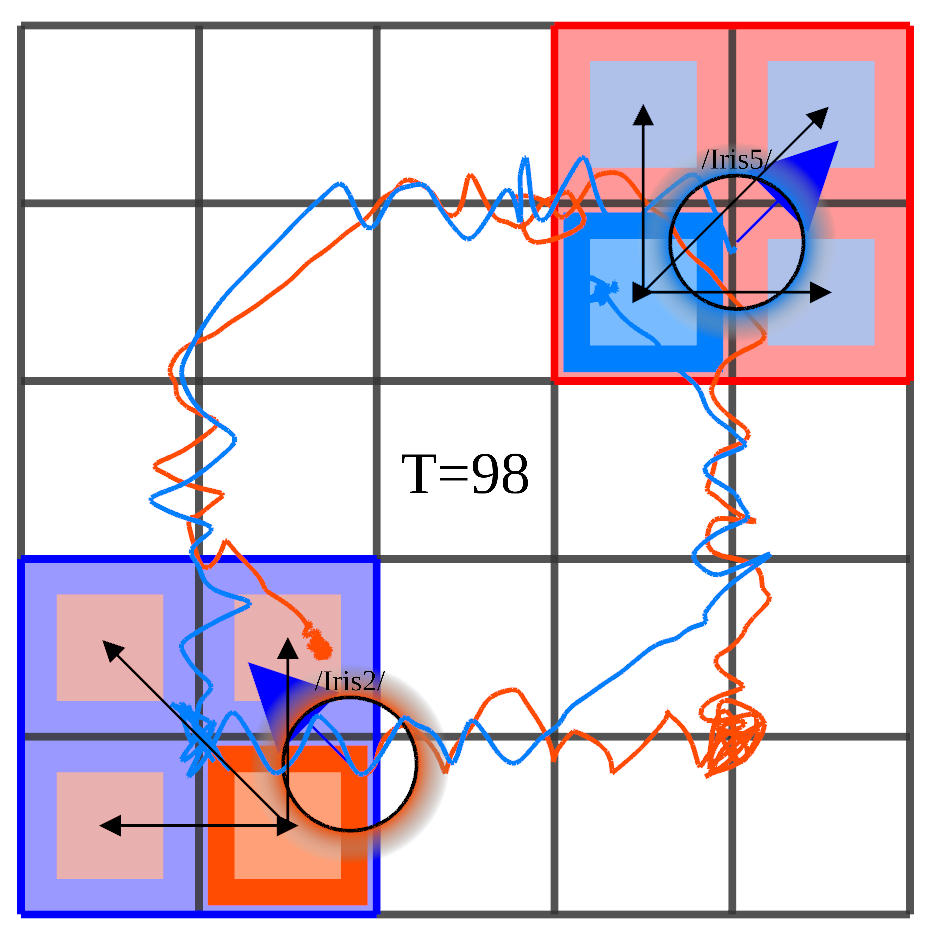
\includegraphics[width=\linewidth]{multi_ltl/multi12}
  \end{minipage} 
\end{figure}
\end{frame}


\begin{frame}
\frametitle{Multi agent experiment - the video}
\end{frame}

%% CONCLUSION
% sum up rapidely what you have done
% say what could be done

\end{document}